\documentclass{beamer}
\mode<presentation> {
%\usetheme{Madrid}
%\usetheme{default}
\usepackage{color}
\definecolor{bottomcolour}{rgb}{0.21,0.11,0.21}
\definecolor{middlecolour}{rgb}{0.21,0.11,0.21}
\setbeamercolor{structure}{fg=white}
\setbeamertemplate{frametitle}[default]%[center]
\setbeamercolor{normal text}{bg=black, fg=white}
\setbeamertemplate{background canvas}[vertical shading]
[bottom=bottomcolour, middle=middlecolour, top=black]
\setbeamertemplate{items}[circle]
\setbeamertemplate{navigation symbols}{} %no nav symbols
\setbeamercolor{block title}{use=structure,fg=white,bg=structure.fg!50!red!50!blue!100!green}
\setbeamercolor{block body}{parent=normal text,use=block title,bg=block title.bg!5!white!10!bg,fg=white}
\setbeamertemplate{navigation symbols}{}
}
\usepackage{graphicx} 
\usepackage{booktabs} 
\usepackage[utf8]{inputenc}  
\usepackage[T1]{fontenc}  
\usepackage{geometry}     
%\usepackage[francais]{babel} 
\usepackage{eurosym}
\usepackage{verbatim}
\usepackage{ragged2e}
\justifying
%%%%%%%%%%%%%%%%%%%%%%%%%%%%%%%%%%%%%%%%%%%%%%%%%%%%%%%%%%%%%%%%
%% ccBeamer 0.1, 2007-07-02                                   %%
%% Written by Sebastian Pipping <webmaster@hartwork.org>      %%
%% ---------------------------------------------------------- %%
%% Licensed under Creative Commons Attribution-ShareAlike 3.0 %%
%% http://creativecommons.org/licenses/by-sa/3.0/             %%
%%%%%%%%%%%%%%%%%%%%%%%%%%%%%%%%%%%%%%%%%%%%%%%%%%%%%%%%%%%%%%%%


%% Images
\newcommand{\CcImageBy}[1]{%
	
\includegraphics[scale=#1]{creative_commons/cc_by_30.pdf}%
}
\newcommand{\CcImageCc}[1]{%
	
\includegraphics[scale=#1]{creative_commons/cc_cc_30.pdf}%
}
\newcommand{\CcImageDevNations}[1]{%
	
\includegraphics[scale=#1]{creative_commons/cc_dev_nations_30.pdf}%
}
\newcommand{\CcImageNc}[1]{%
	
\includegraphics[scale=#1]{creative_commons/cc_nc_30.pdf}%
}
\newcommand{\CcImageNd}[1]{%
	
\includegraphics[scale=#1]{creative_commons/cc_nd_30.pdf}%
}
\newcommand{\CcImagePd}[1]{%
	
\includegraphics[scale=#1]{creative_commons/cc_pd_30.pdf}%
}
\newcommand{\CcImageSa}[1]{%
	
\includegraphics[scale=#1]{creative_commons/cc_sa_30.pdf}%
}
\newcommand{\CcImageSampling}[1]{%
	
\includegraphics[scale=#1]{creative_commons/cc_sampling_30.pdf}%
}
\newcommand{\CcImageSamplingPlus}[1]{%
	
\includegraphics[scale=#1]{creative_commons/cc_sampling_plus_30.pdf}%
}


%% Groups
\newcommand{\CcGroupBy}[1]{% zoom
	\CcImageBy{#1}%
}
\newcommand{\CcGroupByNc}[2]{% zoom, gap
	\CcImageBy{#1}\hspace*{#2}\CcImageNc{#1}%
}
\newcommand{\CcGroupByNcNd}[2]{% zoom, gap
	\CcImageBy{#1}\hspace*{#2}\CcImageNc{#1}\hspace*{#2}\CcImageNd{#1}%
}
\newcommand{\CcGroupByNcSa}[2]{% zoom, gap
	\CcImageBy{#1}\hspace*{#2}\CcImageNc{#1}\hspace*{#2}\CcImageSa{#1}%
}
\newcommand{\CcGroupByNd}[2]{% zoom, gap
	\CcImageBy{#1}\hspace*{#2}\CcImageNd{#1}%
}
\newcommand{\CcGroupBySa}[2]{% zoom, gap
	\CcImageBy{#1}\hspace*{#2}\CcImageSa{#1}%
}
\newcommand{\CcGroupDevNations}[1]{% zoom
	\CcImageDevNations{#1}%
}
\newcommand{\CcGroupNcSampling}[2]{% zoom, gap
	\CcImageNc{#1}\hspace*{#2}\CcImageSampling{#1}%
}
\newcommand{\CcGroupPd}[1]{% zoom
	\CcImagePd{#1}%
}
\newcommand{\CcGroupSampling}[1]{% zoom
	\CcImageSampling{#1}%
}
\newcommand{\CcGroupSamplingPlus}[1]{% zoom
	\CcImageSamplingPlus{#1}%
}


%% Text
\newcommand{\CcLongnameBy}{Attribution}
\newcommand{\CcLongnameByNc}{Attribution-NonCommercial}
\newcommand{\CcLongnameByNcNd}{Attribution-NoDerivs}
\newcommand{\CcLongnameByNcSa}{Attribution-NonCommercial-ShareAlike}
\newcommand{\CcLongnameByNd}{Attribution-NoDerivs}
\newcommand{\CcLongnameBySa}{Attribution-ShareAlike}

\newcommand{\CcNote}[1]{% longname
	This work is licensed under the \textit{Creative Commons #1 3.0 License}.%
}

\title[Firefox OS, l'OS pour smartphone par Mozilla]{Firefox OS, l'OS pour smartphone par Mozilla} 
\date{Capitole du libre - 21-22 novembre 2015}
\author{Genma}
\begin{document}
\begin{frame}
	\titlepage
	\begin{center}		
	
\includegraphics[scale=0.2]{./images/firefox-os.jpg}
		\\	
	\CcGroupByNcSa{0.83}{0.95ex}\\[2.5ex]
		{\tiny\CcNote{\CcLongnameByNcSa}}
		\vspace*{-2.5ex}
	\end{center}
\end{frame}

\begin{frame}
\frametitle{
\includegraphics[scale=0.4]{./images/Genma.jpg} \ \ \  A propos de moi  }
\begin{columns}[c] 
\column{.55\textwidth} 
\textbf{Où me trouver sur Internet?}
\begin{itemize}
\item Le Blog de Genma : http://genma.free.fr
\item Twitter : http://twitter.com/genma
\end{itemize}

\column{.5\textwidth} 
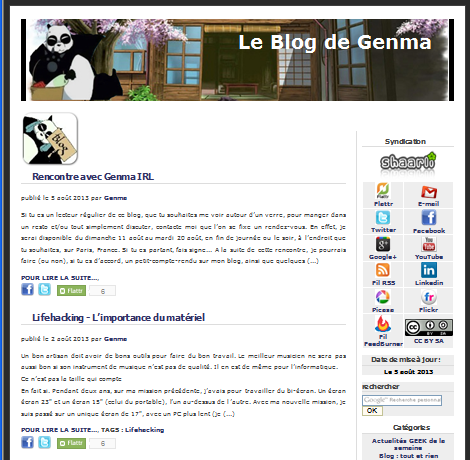
\includegraphics[width=5cm,height=5cm]{./images/blog.png} 
\end{columns}
\end{frame}

%----------------------------------------------------------------------------------------
\begin{frame}
\frametitle{Remerciements}
\justifying{
Je remercie la communauté francophone autour de Firefox OS pour les builds communautaires 
\url{http://builds.firefoxos.mozfr.org/}
le support, les billets de blog, la promotion de FFOS.\\
Ainsi que Mozilla pour avoir lancé FFOS.
}
\end{frame}
%----------------------------------------------------------------------------------------
\begin{frame}
\begin{center}
\Huge{Introduction}
\\~\\

\includegraphics[scale=0.3]{./images/firefox-os.jpg}
\end{center}
\end{frame}

\begin{frame}
\frametitle{Mozilla - De Firefox à FirefoxOS}
\justifying{
En 2004, Mozilla a lancé Firefox, le navigateur web gratuit et
désintéressé pour votre ordinateur.
\\~\\
En 2014, Mozilla introduit en France Firefox OS, le système d’
exploitation respectueux de votre vie privée pour votre téléphone.
}
\end{frame}
%---------------------------------------------------------------------------------------
\begin{frame}
\frametitle{FirefoxOS - un OS libre}
\justifying{
Firefox OS est conçu par une communauté internationale de bénévoles, et de développeurs situés dans plusieurs pays, notamment dans les bureaux de Mozilla Paris.
\\~\\
Le logiciel est libre : Firefox OS est un logiciel libre, sans secrets, auditable. Tout le code source est ouvert et disponible.
}
\end{frame}

%----------------------------------------------------------------------------------------
\begin{frame}
\begin{center}
\Huge{Architecture}
\\~\\

\includegraphics[scale=0.3]{./images/firefox-os.jpg}
\end{center}
\end{frame}
%---------------------------------------------------------------------------------------
\begin{frame}
\frametitle{Architecture de FFOS}
\begin{center}
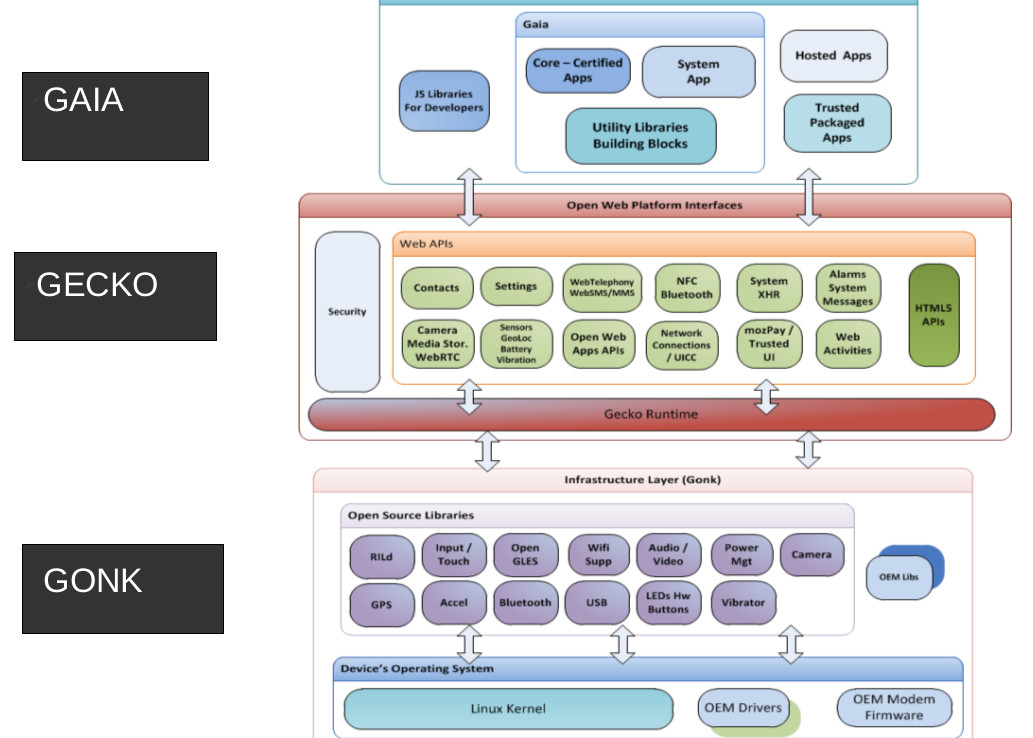
\includegraphics[scale=0.3]{./images/ffos_architecture.jpg}
\end{center}
\end{frame}

\begin{frame}
\begin{center}
\includegraphics[scale=0.06]{./images/Firefox_Layers.jpg}
\end{center}
\end{frame}
%---------------------------------------------------------------------------------------
\begin{frame}
\frametitle{Architecture de FFOS}
\begin{block}{Gaia - l'interface}
\justifying{Gaia a le rôle d'interface utilisateur de Firefox OS et contrôle tout ce qui interagit avec l'écran.}
\end{block}
\begin{block}{Gecko - le moteur}
\justifying{
Gecko est l'application permettant d'exécuter Firefox OS. Il permet le support des trois standards : HTML, CSS et JavaScript.}
\end{block}
\begin{block}{Gonk - le noyau}
\justifying{Gonk consiste en un noyau Linux et une couche d'abstraction matérielle de l'espace utilisateur (HAL).}
\end{block}
\end{frame}

%----------------------------------------------------------------------------------------
\begin{frame}
\begin{center}
\Huge{Quelles applications?}
\\~\\

\includegraphics[scale=0.3]{./images/logo_marketplace.png}
\end{center}
\end{frame}

\begin{frame}
\frametitle{Les applications par défaut dans FFOS}
\begin{columns}[c] 
\column{.55\textwidth} 
\begin{block}{Les fonctionnalités d'un smartphone}
\begin{itemize}
\item Téléphone
\item Contacts
\item SMS/MMS
\item Agenda
\item Mail
\item Firefox comme navigateur
\item ...
\end{itemize}
\end{block}
\column{.5\textwidth} 
\begin{center}
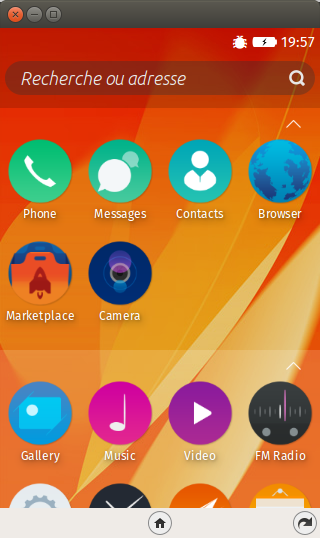
\includegraphics[scale=0.45]{./images/capture.png} 
\end{center}
\end{columns}
\end{frame}

\begin{frame}
\frametitle{Les appplications pour FFOS}
Les applications sont toutes en HTML5/CSS3/Javascript
\begin{itemize}
\item N'importe qui peut en développer une.
\item Toutes ne sont pas libres.
\end{itemize}

\begin{center}
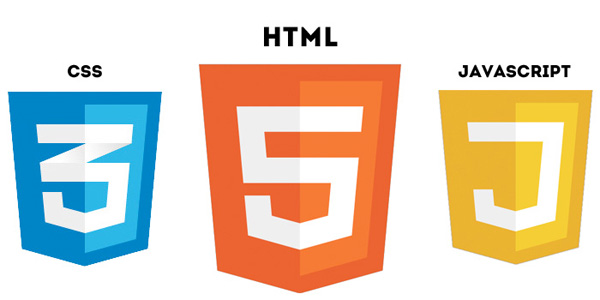
\includegraphics[scale=0.3]{./images/logo-html5.jpg} 
\end{center}
\end{frame}

\begin{frame}
\frametitle{Le marketplace}
\begin{center}
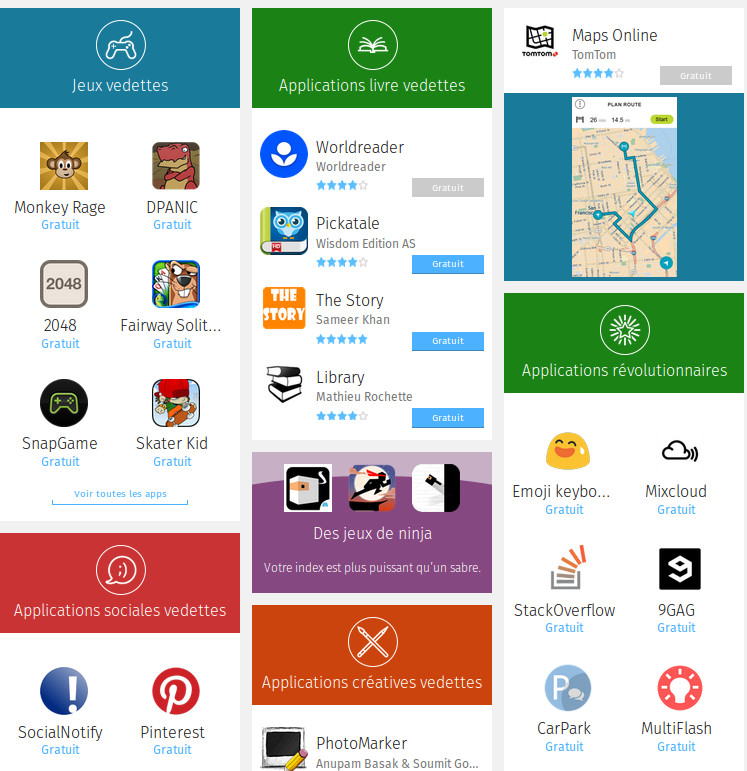
\includegraphics[scale=0.3]{./images/marketplace01.jpg}
\end{center}
\end{frame}

\begin{frame}
\frametitle{Les permissions des applications}
\begin{center}
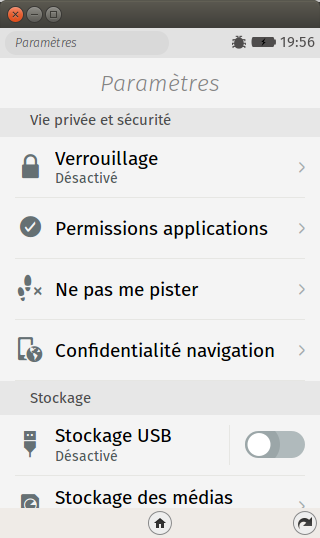
\includegraphics[scale=0.5]{./images/Screenshot01.png}
\end{center}
\end{frame}

%----------------------------------------------------------------------------------------
\begin{frame}
\begin{center}
\Huge{Quel matériel?}
\\~\\
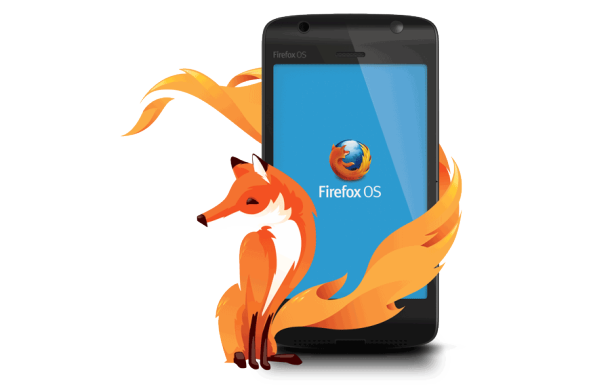
\includegraphics[scale=0.3]{./images/FirefoxOS-logo_610x385.png}
\end{center}
\end{frame}
%---------------------------------------------------------------------------------------
\begin{frame}
\frametitle{Les smartphones existants}
\justifying{
En décembre 2014, on dénombre 14 opérateurs qui commercialisent dans 28 pays à travers le monde des téléphones ayant comme système d'exploitation Firefox OS.}
\begin{itemize}
\item Le ZTE Open C
\item Le Flame
\item Autres téléphones...
\end{itemize}
\begin{center}
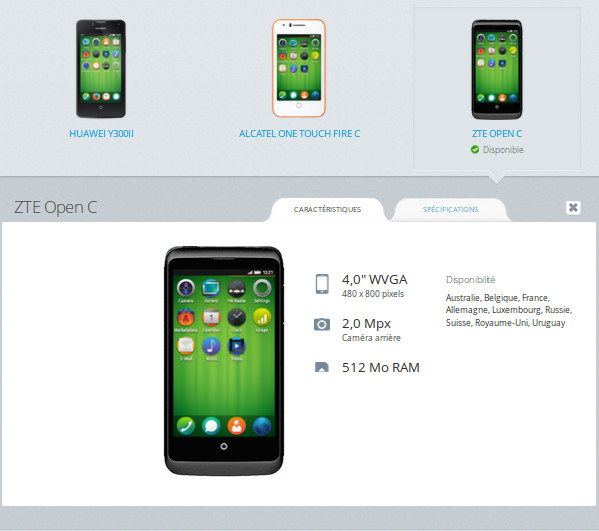
\includegraphics[scale=0.3]{./images/smartphone01.jpg}
\end{center}
\end{frame}
%---------------------------------------------------------------------------------------
\begin{frame}
\frametitle{Les smartphones compatibles}
\begin{block}{Firefox OS est compatible avec un certain nombre d'appareils}
\justifying{
Samsung Nexus S, le Samsung Nexus S 4G, le Samsung Galaxy S II, le Samsung Galaxy Nexus, le Nexus 4 et d'autres.
}
\end{block} 
\begin{block}{Sony Xperia Z3, Z3c }
\justifying{
Des portages sur des modèles Sony sont en cours de réalisation 
\\ Voir \emph{Build and Run Firefox OS on Sony Open Devices}\\
}
\url{https://hacks.mozilla.org/2015/10/build-and-run-firefox-os-on-sony-open-devices/}\end{block} 
\begin{block}{Liste device compatible 2.5} 
\url{https://www.ethercalc.org/HW_support_of_Firefox_OS_2.5_V2}
\end{block} 
\end{frame}

%---------------------------------------------------------------------------------------
\begin{frame}
\frametitle{Les télévisions}
\begin{block}{Panasonic TX-65CR852}
\justifying{

}
\end{block} 
\end{frame}
%----------------------------------------------------------------------------------------
\begin{frame}
\begin{center}
\Huge{Nouveautés de la version 2.5}
\\~\\

\includegraphics[scale=0.3]{./images/firefox-os.jpg}
\end{center}
\end{frame}

%----------------------------------------------------------------------------------------
\begin{frame}
\frametitle{2.5, Spark ?}

\begin{block}{Branche 2.5}
\justifying{
La version 2.5 correspond à la branche du code source pour les couches Gecko (le moteur) et Gaia (l’interface et les applications fournies par défaut).
}
\end{block} 

\begin{block}{Spark}
\justifying{
Spark est un ensemble d’outils, personnalisations et fonctionnalités intégrées. \\~\\Spark est destiné à permettre aux utilisateurs de personnaliser leur expérience, de hacker tout ce qu’ils veulent dans le code source.
}
\end{block} 
\end{frame}

%----------------------------------------------------------------------------------------
\begin{frame}
\frametitle{Le Bureau}
\begin{center}	
\begin{columns}[t]
\begin{column}{5cm}
Les icônes des applications (Téléphone, Mail etc.)\\~\\
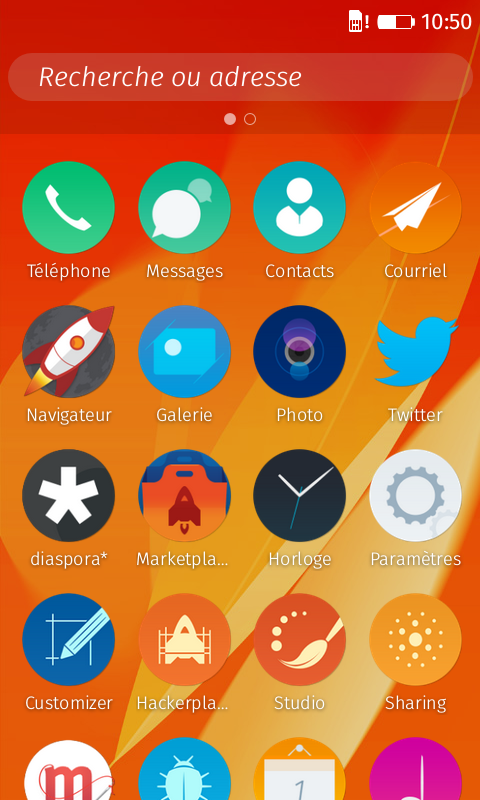
\includegraphics[scale=0.25] {./images/FFOS_Defaut.png} 
\end{column}
\begin{column}{5cm}
0n épingle des pages, des favoris\\~\\
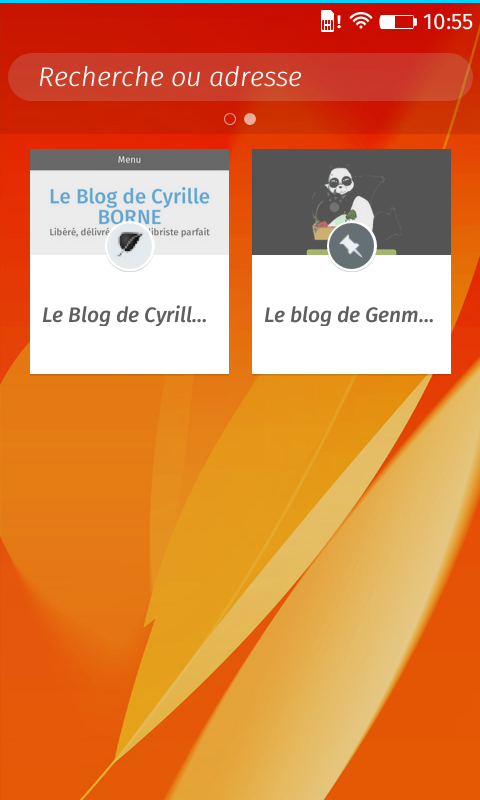
\includegraphics[scale=0.25] {./images/FFOS_Favori.png} 
\end{column}
\end{columns}  
\end{center}
\end{frame}

%----------------------------------------------------------------------------------------
\begin{frame}
\frametitle{La Personnalisation}
\begin{columns}[T]
\begin{column}{5cm}
\begin{block}{Customizer}
\justifying{
peut être utilisé pour créer une application toute entière à partir de zéro, si vous le désirez. Il est livré avec des modèles (templates) sur lesquels vous pouvez commencer votre travail et des widgets que vous pouvez embarquer dans vos applications.
}
\end{block} 
\end{column}
\begin{column}{5cm}
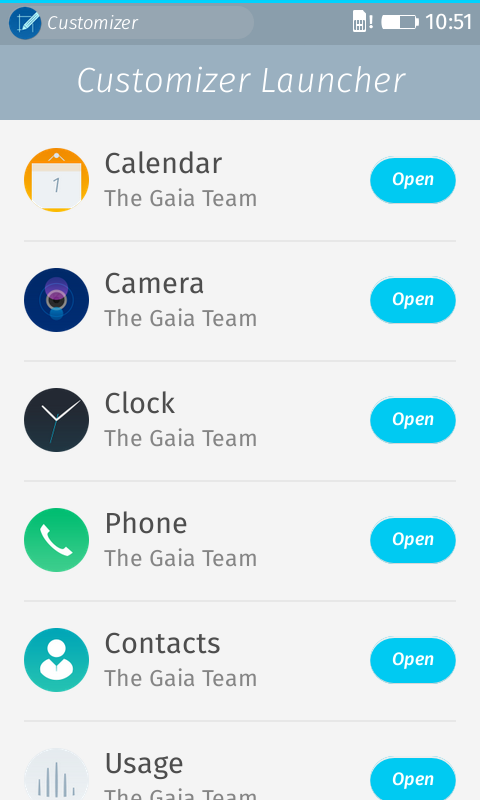
\includegraphics[scale=0.25] {./images/FFOS_Customizer.png} 
\end{column}
\end{columns}  
\end{frame}

%----------------------------------------------------------------------------------------
\begin{frame}
\frametitle{Hackerplace}
\begin{columns}[T]
\begin{column}{5cm}
\begin{block}{Le Hackerplace}
\justifying{
est un marketplace pour des applications et modules complémentaires plus expérimentaux qui n’ont pas encore été approuvés pour le Marketplace. 
\\~\\Il se concentre sur des bidouillages cool que les membres de la communauté ont produits et sur des applications remplaçables.
}
\end{block} 
\end{column}
\begin{column}{5cm}
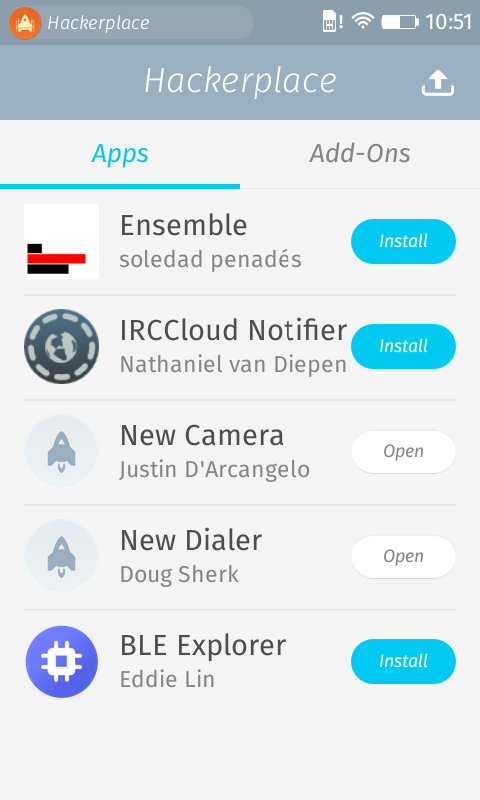
\includegraphics[scale=0.25] {./images/FFOS_HackerSpace.png} 
\end{column}
\end{columns}  
\end{frame}
%----------------------------------------------------------------------------------------
\begin{frame}
\frametitle{P2P Sharing}
\begin{columns}[T]
\begin{column}{5cm}
\begin{block}{Le partage en P2P}
\justifying{
est une application pour découvrir rapidement des personnes à proximité et partager des applications, des modules complémentaires et des thèmes avec eux via Wi-Fi et WiFi Direct.
}
\end{block} 
\end{column}
\begin{column}{5cm}
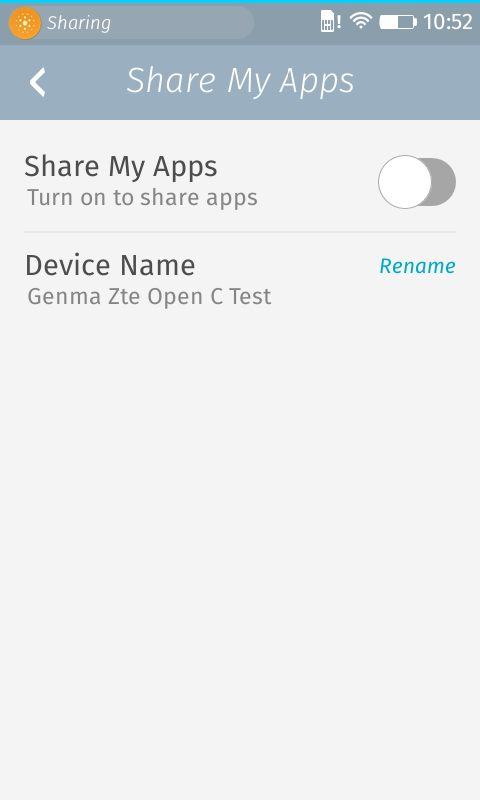
\includegraphics[scale=0.25] {./images/FFOS_ShareApps.png} 
\end{column}
\end{columns}  
\end{frame}
%----------------------------------------------------------------------------------------
\begin{frame}
\frametitle{L'éditeur de thèmes 1/2}
\begin{columns}[T]
\begin{column}{5cm}
\begin{block}{Theme Editor}
\justifying{
est une application pour gérer les thèmes de votre appareil, par exemple en modifiant le texte, le fond et les couleurs des composants dans tout l’appareil.
}
\end{block} 
\end{column}
\begin{column}{5cm}
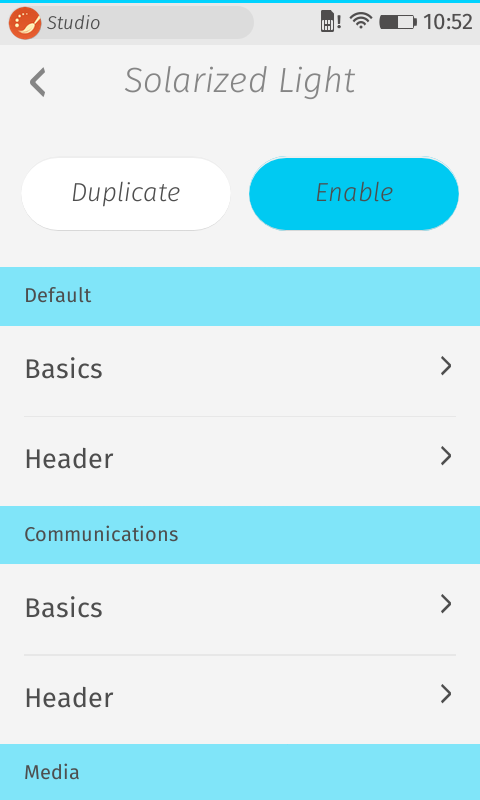
\includegraphics[scale=0.25] {./images/FFOS_Theme01.png} 
\end{column}
\end{columns}  
\end{frame}

\begin{frame}
\frametitle{L'éditeur de thèmes 2/2}
\begin{columns}[T]
\begin{column}{5cm}
\begin{block}{Theme Editor}
\justifying{
est une application pour gérer les thèmes de votre appareil, par exemple en modifiant le texte, le fond et les couleurs des composants dans tout l’appareil.
}
\end{block} 
\end{column}
\begin{column}{5cm}
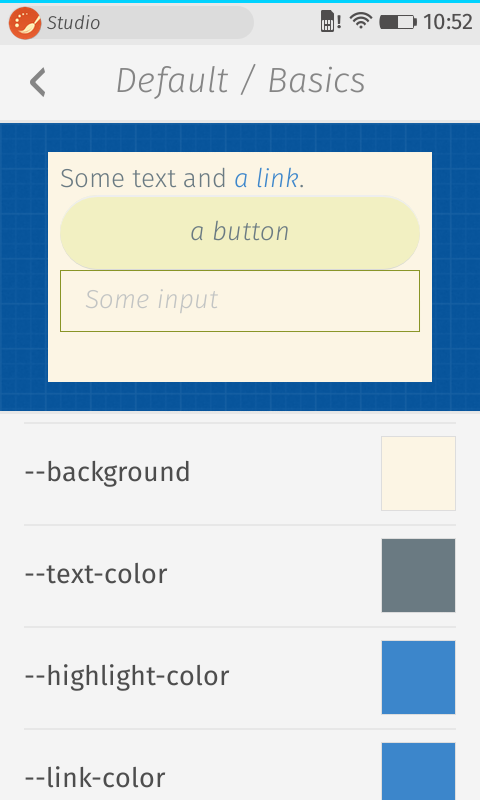
\includegraphics[scale=0.25] {./images/FFOS_Theme02.png} 
\end{column}
\end{columns}  
\end{frame}
%----------------------------------------------------------------------------------------
\begin{frame}
\frametitle{Entraide via des questions réponses}
\begin{columns}[T]
\begin{column}{5cm}
\begin{block}{BuddyUp}
\justifying{
est un service pour poser des questions et obtenir des réponses de membres de la communauté. Vous pouvez également être de l’autre côté et répondre aux questions des utilisateurs.
}
\end{block} 
\end{column}
\begin{column}{5cm}
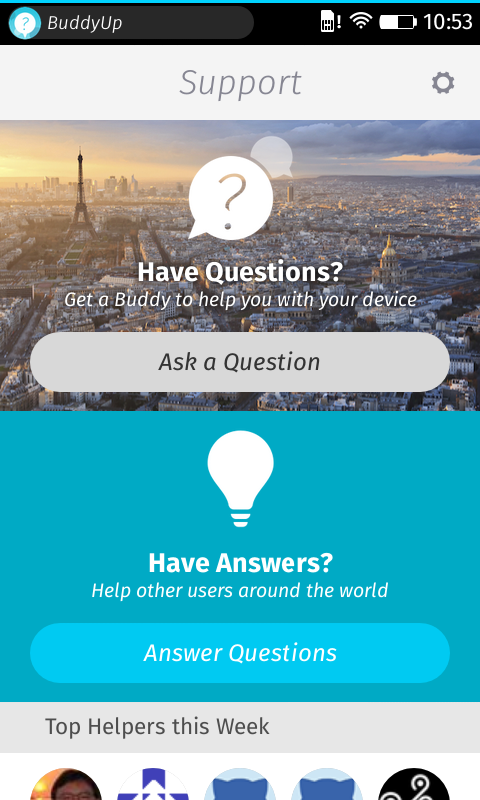
\includegraphics[scale=0.25] {./images/FFOS_Support.png} 
\end{column}
\end{columns}  
\end{frame}
%----------------------------------------------------------------------------------------
\begin{frame}
\frametitle{Apprendre et développer}
\begin{columns}[T]
\begin{column}{5cm}
\begin{block}{Webmaker}
\justifying{
est une application qui facilite la création de choses sur le Web, à savoir faire vos propres pages web, vidéos interactives, remix, applications mobiles et de plus – apprendre sur le tas les mécaniques du Web, le code et d’autres compétences précieuses.
}
\end{block} 
\end{column}
\begin{column}{5cm}
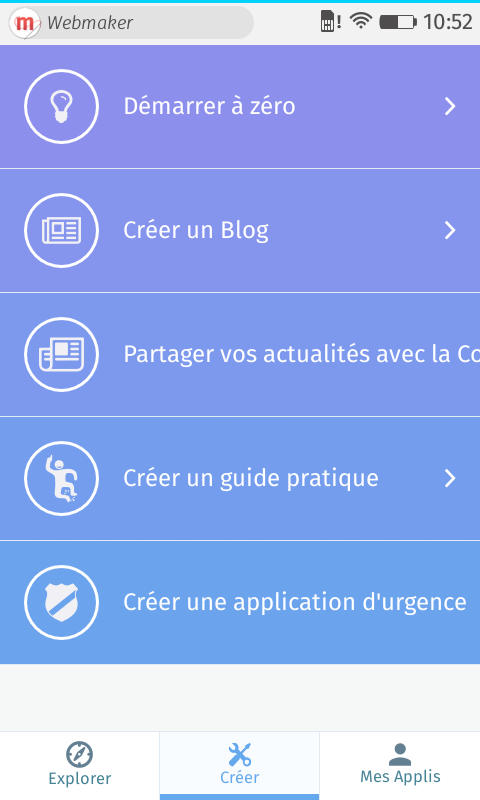
\includegraphics[scale=0.25] {./images/FFOS_Webmaker.png} 
\end{column}
\end{columns}  
\end{frame}
%----------------------------------------------------------------------------------------
\begin{frame}
\frametitle{Remplacer les applications existantes}
\begin{columns}[T]
\begin{column}{5cm}
\begin{block}{Via les applications du Hackerspace}
\justifying{
Toutes les applications système telles que les applications numéroteur, messages, contacts, etc. sont remplaçables.
}
\end{block} 
\end{column}
\begin{column}{5cm}
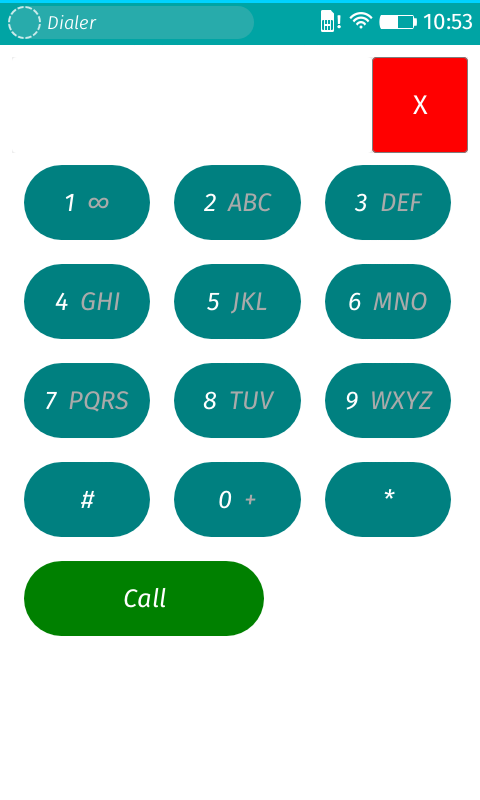
\includegraphics[scale=0.25] {./images/FFOS_Dialer.png} 
\end{column}
\end{columns}  
\end{frame}
%----------------------------------------------------------------------------------------
\begin{frame}
\frametitle{S'informer}
\begin{columns}[T]
\begin{column}{5cm}
\begin{block}{}
\justifying{

}
\end{block} 
\end{column}
\begin{column}{5cm}
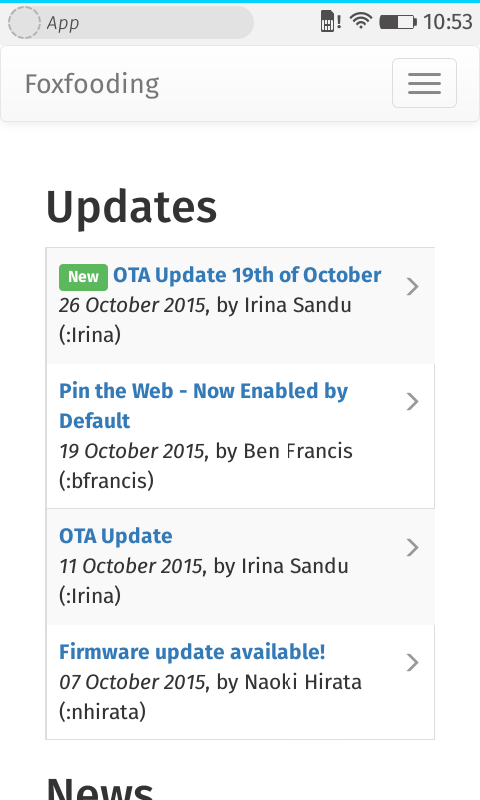
\includegraphics[scale=0.25] {./images/FFOS_FoxFooding.png} 
\end{column}
\end{columns}  
\end{frame}
%----------------------------------------------------------------------------------------
\begin{frame}
\frametitle{Client IRC}
\begin{columns}[T]
\begin{column}{5cm}
\begin{block}{}
\justifying{

}
\end{block} 
\end{column}
\begin{column}{5cm}
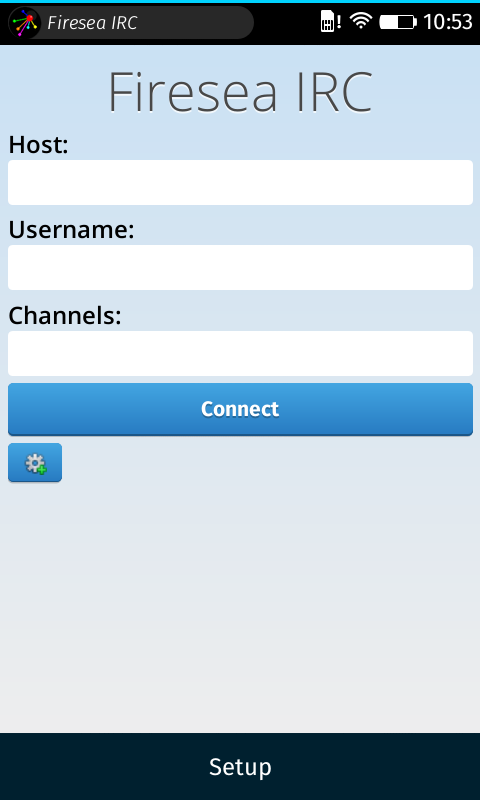
\includegraphics[scale=0.25] {./images/FFOS_IRC.png} 
\end{column}
\end{columns}  
\end{frame}
%----------------------------------------------------------------------------------------

%----------------------------------------------------------------------------------------
\begin{frame}
\begin{center}
\Huge{Où trouver des informations \\ sur FFOS?}
\end{center}
\end{frame}
\begin{frame}
\frametitle{Où trouver des informations sur FFOS?}
\begin{itemize}
\item Le site officiel par Mozilla \url{https://www.mozilla.org/fr/firefox/os/}
\item Le forum de Mozilla-fr \url{https://forums.mozfr.org}
\item Les mailing-listes \url{http://mozfr.org/participer}
\item Bugzilla \url{https://bugzilla.mozilla.org}
\item Les blogs de la communauté \url{http://mozfr.org}
\item Twitter/Diaspora-Framasphère via \#FirefoxOS
\end{itemize}
\end{frame}

%----------------------------------------------------------------------------------------
\begin{frame}
\begin{center}
\Huge{Les builds communautaires}
\\~\\
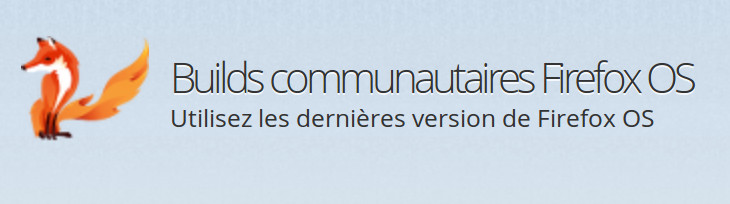
\includegraphics[scale=0.3]{./images/builds_communautaire_logo.jpg}
\end{center}
\end{frame}
%---------------------------------------------------------------------------------------
\begin{frame}
\frametitle{Les builds communautaires de FirefoxOS}
\begin{center}
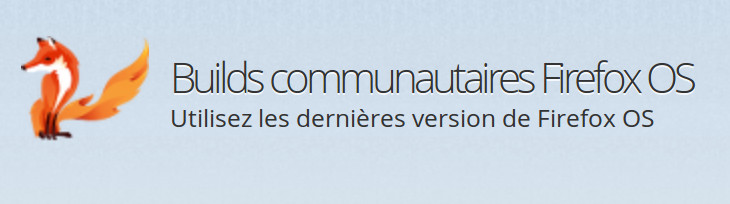
\includegraphics[scale=0.3]{./images/builds_communautaire_logo.jpg}
\\~\\
\url{http://builds.firefoxos.mozfr.org/}
\\
\url{http://builds.firefoxos.mozfr.org/doc/fr/maj-firmware-modem}
\\~\\
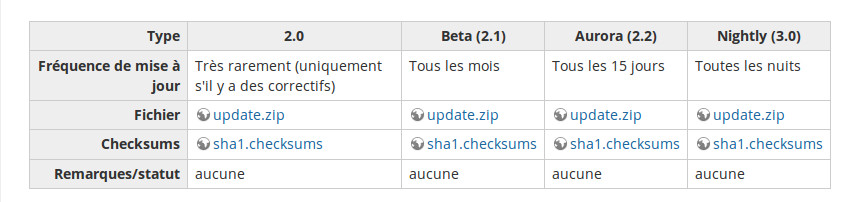
\includegraphics[scale=0.3]{./images/builds_communautaire_01.jpg}
\end{center}
\end{frame}
%---------------------------------------------------------------------------------------

\begin{frame}
\frametitle{Les builds communautaires de FirefoxOS}

\justifying{Comme le code est ouvert/disponible, la communauté construit des builds (des ROMS).}

\begin{block}{Différentes branches}
\begin{itemize}
\item Beta : 2.1
\item Aurora : 2.2
\item Nighty Build : 3.0
\end{itemize}
\end{block}

\begin{block}{Les avantages des builds communautaires}
\begin{itemize}
\justifying{
\item Relativement stable
\item Communauté réactive et sympathique. 
\item Permet d'avoir des fonctionnalités plus évoluées que la ROM par défaut.
}
\end{itemize}
\end{block}
\end{frame}

\begin{frame}
\begin{block}{Les limites des builds communautaires}\begin{itemize}
\justifying{
\item Les bugs ne sont pas du fait de l’équipe qui s’occupe de mettre à disposition les builds. Ils sont remontés aux développeurs et on ne peut faire autre chose qu’attendre une nouvelle compilation en espérant que le problème ait été réglé entre temps.
\item La fréquence des mises à jour, elle est donnée à titre indicatif mais ne doit pas être prise au pied de la lettre.
}
\end{itemize}
\end{block}
\end{frame}


%----------------------------------------------------------------------------------------
\begin{frame}
\begin{center}
\Huge{Contribuer à FFOS?}
\\~\\

\includegraphics[scale=0.3]{./images/firefox-os.jpg}
\end{center}
\end{frame}
%----------------------------------------------------------------------------------------
\begin{frame}
\frametitle{Tester FFOS}
Le simulateur de FFOS dans Firefox le navigateur. 

\begin{center}
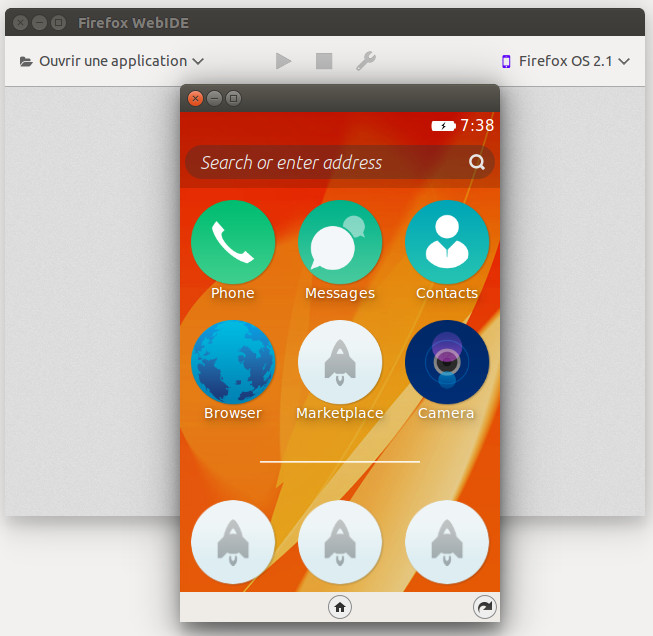
\includegraphics[scale=0.3]{./images/ffos_simulator.jpg}
\end{center}
\justifying{
Une fois l'extension installée, Menu Outil>Développement web >Web ide (MAJ+F8).
Cela donne un aperçu de ce qu'est FirefoxOS.
}
\end{frame}

%----------------------------------------------------------------------------------------
\begin{frame}
\frametitle{Développer pour FFOS}
\justifying{
La documentation MDN est bien faite, assez complète.\\
\url{https://developer.mozilla.org/fr/docs/Mozilla/Boot_to_Gecko/Writing_apps_for_Boot_to_Gecko}
\\
Il est possible de télécharger des applications existantes et de regarder leur code source, pour apprendre, comprendre...
\\
Tout le code source est disponible sur Github.
}
\end{frame}

%----------------------------------------------------------------------------------------
\begin{frame}
\begin{center}
\Huge{Passer à FFOS ou attendre?}
\\~\\

\includegraphics[scale=0.3]{./images/firefox-os.jpg}
\end{center}
\end{frame}
%----------------------------------------------------------------------------------------

\begin{frame}
\frametitle{Passer à FFOS ou attendre?}
\begin{block}{Si on est Android/IOS addict}
\justifying{
NON. Car il y aura \textit{forcément} l'application indispensable dont on ne peut se passer...
}
\end{block}

\begin{block}{Geek curieux, libriste ou 1er Smartphone}
\begin{itemize}
\justifying{
\item Oui, mais avec un build communautaire. 
\item Attendre la sortie du ZTE Open L.
}
\end{itemize}
\end{block}

\begin{block}{Ce qu'il me manque dans FFOS}
\begin{itemize}
\justifying{
\item Le chiffrement du stockage (SD-Card)
\item Des applications comme Textsecure…
\item Le TorBrowser (c'est prévu)
\item L'absence de CardDAV
}
\end{itemize}
\end{block}
\end{frame}

%----------------------------------------------------------------------------------------
\begin{frame}
\begin{center}
\Huge{FFOS Bilan}
\\~\\

\includegraphics[scale=0.3]{./images/firefox-os.jpg}
\end{center}
\end{frame}
%----------------------------------------------------------------------------------------

\begin{frame}
\frametitle{FFOS Bilan}
\begin{block}{Les plus}
\begin{itemize}
\justifying{
\item C'est le système le plus libre, le plus ouvert et le seul à n'être pas développé par une entreprise commerciale.
\item Les builds communautaires et la communauté.
\item OS libre (aux blobs proprios/drivers près pour le noyau).
\item TOUT EST WEB (HTML5/CSS3/Javascript).
}
\end{itemize}
\end{block}

\begin{block}{Les moins}
\begin{itemize}
\justifying{
\item OS jeune (bugs, manque de fonctionnalités).
\item Constructeurs frileux et de ce fait pas de smartphone moyen ou haut de gamme.
}
\end{itemize}
\end{block}
\end{frame}

%---------------------------------------------------------------------------------------
\begin{frame}
\begin{center}
\Huge{Questions et discussion}
\\~\\

\includegraphics[scale=0.3]{./images/firefox-os.jpg}
\end{center}
\end{frame}

%======================================================
\begin{frame}
\begin{center}
\Huge{ANNEXES}
\end{center}
\end{frame}

%---------------------------------------------------------------------------------------
\begin{frame}
\frametitle{Architecture de FFOS - Détaillée 1/3}
\begin{block}{Gonk - le noyau}
\justifying{Gonk consiste en un noyau Linux et une couche d'abstraction matérielle de l'espace utilisateur (HAL)}.
\begin{itemize}
\item Couche basse
\item Kernel Linux + Matériels
\item Hardware
\item libre ou propriétaire
\item Abstraction Layer (HAL)
\item Pas exposé le JS
\item Isolé de Gaia
\item Communication par Gecko
\end{itemize}
\end{block}
\end{frame}

\begin{frame}
\frametitle{Architecture de FFOS - Détaillée 2/3}
\begin{block}{Gecko - le moteur}
\justifying{
Gecko est l'application permettant d'exécuter Firefox OS. Il permet le support  des trois standards : HTML, CSS et JavaScript}.
\begin{itemize}
\item Moteur de rendu HTML5
\item Gestion des API
\item De plus en plus complet
\item Exécution des applications (runtime)
\item Mécanisme de lancement dans Firefox pour HTML 5, CSS et Javascript
\end{itemize}
\end{block}
\end{frame}

\begin{frame}
\frametitle{Architecture de FFOS - Détaillée 3/3}
\begin{block}{Gaia - l'interface}
\justifying{Gaia a le rôle d'interface utilisateur de Firefox OS et contrôle tout ce qui interagit avec l'écran}.
\begin{itemize}
\item Interface utilisateur (IHM)
\item Construction API Full Web
\item HTML 5 + open Web
\item Communique avec Geckovia des Web API
\item Les Apps sont exécutés enmode sandbox
\item Offline
\item LocalStorage, appCache
\end{itemize}
\end{block}
\end{frame}

%---------------------------------------------------------------------------------------
\begin{frame}
\frametitle{phoxygen}
\url{http://www.phoxygen.com/}
\end{frame}

%---------------------------------------------------------------------------------------
\begin{frame}
\frametitle{Les applications - Mon usage}
\begin{columns}[c] 
\column{.55\textwidth} 
\begin{itemize}
\item Téléphone (Appel/SMS)
\item Mail
\item Agenda
\item Twitter/Diaspora
\item Lecteur RSS
\item Consultation de site version mobile
\end{itemize}
Une sorte de mini-tablette, pour un usage ponctuel.
\column{.5\textwidth} 
\begin{center}
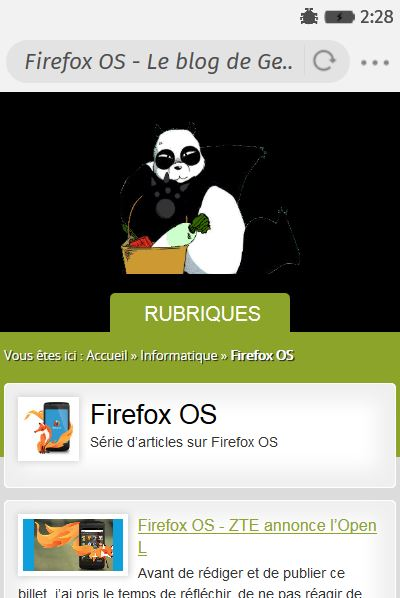
\includegraphics[scale=0.6]{./images/site_version_mobile.jpg} 
\end{center}
\end{columns}
\end{frame}
%---------------------------------------------------------------------------------------
\end{document}
